%!TEX root = ../physical-olympics-2.tex
\chapter{相与相变摘要}


\section{相平衡}

我们此前介绍过的单组分理想气体体系属于\emph{单元单相系}(uni-component-multi-phase system). 而混合理想气体则属于\emph{多元单相系}(multi-component-uni-phase system). \emph{相}(phase)指各强度量代表的宏观属性在空间与时间分布上均匀的物质形式. \emph{相变}(phase transition)指不同相在一定条件下发生转变的热学过程, 这个过程往往同时伴随着体积变化与吸热. 而其中准静态的相变过程又具有特殊的研究价值. 在准静态的相变过程中, 转变的两相之间彼此达到热平衡, 互相之间没有自发转变的倾向. 最终相变的方向为何? 实际上这与环境到体系传递的热量有关. 实际上如果考虑相一到相二的每一摩尔的转变, 我们定义\emph{相变潜热}(latent heat): 指等温等压条件下的吸热, 所以也是摩尔焓的增量:
\[Q=\nu l=h_2-h_1=u_2-u_1+p(v_2-v_1)\]

它的正负取决于两相本身. 一般来说固相到液相, 液相到气相是吸热的, 相变潜热$l>0$. 比如, $0\cdgr$下若把水的比热容记做$1{\rm cal/g\cdot K}$,\,那么水的溶解热与汽化热为$80{\rm cal/g}$与$600{\rm cal/g}$,\,$100\cdgr$下汽化热降低到只有$540{\rm cal/g}$.\,冰和水蒸气的比热容几乎刚好只有水的一半$0.5{\rm cal/g\cdot K}$.

在不吸热不放热时, 相变无从得以发生. 此时相平衡的研究变得格外重要. 最复杂的情况为\emph{多元多相系}(multi-component-multi-phase system). 比如糖水和糖块的平衡, 两相中溶液相中存在两种不同的分子(二元)但是又分出了两个明确的相. 而实际情况是, 研究\emph{单元二相系}(uni-component-bi-phase system)的足以揭示其中的关键结论.

此前已经写出热力学基本关系式:
\[\ud U=T\ud S-p\ud V+\mu \ud N\]

这样我们可以得到熵变与$U,\,V,\,N$的关系:
\[\ud S=\frac{\ud U}{T}+\frac{p}{T}\ud V -\frac{\mu}{T}\ud N\]

对于二相平衡系统, 设想一个一般的过程, 熵变应该是:
\[\ud S=\left(\frac{\ud U_2}{T_2}+\frac{\ud U_1}{T_1}\right)+\left(\frac{p_2}{T_2}\ud V_2+\frac{p_1}{T_1}\ud V_1\right)+\left(\frac{\mu_2}{T_2}\ud N_2+\frac{\mu_1}{T_1}\ud N_1\right)\]

我们知道, 一个典型的两相平衡系统必须温度相等:
\[T_1=T_2\]

现在看来这一项有了另一种理解方式: 当我们限制$\ud V_1=\ud V_2=0,\,\ud N_1=\ud N_2=0$时, 两相只能从外界吸热. 再命$\ud U_1=-\ud U_2$, 这就是说两相之间有传热而不从外界吸热. 那么根据熵增原理, 非平衡态时:
\[\ud S=\ud U_2\left(\frac{1}{T_2}-\frac{1}{T_1}\right)>0\]

可见, 当且仅当$T_1>T_2$时二相可以向一相放热. 而温度相等后则达到两相平衡态.

类似地, 我们可以处理压强相等做为两相平衡系统的条件:
\[p_1=p_2\]

这是因为设想已经知道$T_1=T_2=T$. 再考虑$\ud N_1=\ud N_2=0$的情况, 但是两个相不仅不从外界吸热, 总体积还不变, 同时也允许两相间的吸放热和各自做膨胀与收缩. 那么同样符合熵增原理:
\[\ud S=\ud U_2\left(\frac{1}{T}-\frac{1}{T}\right)+(p_2-p_1)\frac{\ud V_2}{T}>0\]

可见, 当且仅当$p_2>p_1$时二相可以膨胀并压缩一相. 而压强相等后则达到两相平衡态.

我们已经说明了, 相平衡是等温等压下的共存. 而继续分析可以给出\emph{相平衡条件}(phase equilibrium condition). 设想已经知道$T_1=T_2=T,\, p_1=p_2=p$. 但是考虑两相之间交换粒子的情况. 同时进一步要求体系绝热且总体积不变(相当于等温等压相变后整体发生绝热膨胀或压缩). 熵增原理给出:
\[\ud S=\ud U_2\left(\frac{1}{T}-\frac{1}{T}\right)+(p-p)\frac{\ud V_2}{T}+(\mu_1-\mu_2)\frac{\ud N_2}{T}>0\]

可见. 当且仅当$\mu_2<\mu_1$时, 一相的粒子会自发地向二相转移. 而能够两相共存的相平衡条件就应该是:
\[\mu_1(T,\,p)=\mu_2(T,\,p)\]

我们称温度相等, 压强相等, 化学势相等的三个条件分别为热学平衡, 力学平衡与化学平衡条件.

关于相平衡条件(化学平衡条件)我们可以直接推广到多元多相系和非平衡情况. 例如在饱和糖水溶液和糖块的共存情况下. 我们应当可以根据微观方法计算出糖块中每糖分子的化学势$\mu_1$和糖水中每糖分子的化学势$\mu_2$. 那么由于饱和糖水与糖块的共存是一个平衡态, 推断两个化学势必须相等$\mu_1=\mu_2$. 而如果升温使得糖水不再饱和, $\mu_2$就会下降到比$\mu_1$低, 正如``化学势''这一称呼所暗示的那样, 化学势高的糖块中的糖分子就会向化学势低的糖水中自发转移. 反之, 如果降温使得糖水过饱和, $\mu_2$就会上升到比$\mu_1$高, 糖块就会由于沉积相变而增大.

两相平衡的化学势必须相等这个条件是令人觉得新奇的. 我们知道, 若取摩尔化学势. 那么其定义式:
\[\mu=u-Ts+pv\]

我们要处理的相变一般是\emph{一级相变}(first order phase transition). 此时, 两相的摩尔内能$u$, 摩尔熵$s$, 摩尔体积$v$都是不相等的:
\[u_1\neq u_2 \quad,\quad s_1\neq s_2 \quad,\quad v_1\neq v_2\]

但是, 化学势却要相等:
\[u_1-Ts_1+pv_1=u_2-Ts_2+pv_2\]

实际上, 上式正是:
\[l=h_2-h_1=(u_2+pv_2)-(u_1+pv_1)=T(s_2-s_1)\]

从而相变平衡条件实际上就是说相变吸热恰好对应了体系的熵增这一准静态过程符合的条件, 也就不再神秘了.

但最后值得一提, 一定压强下, 随温度升高降低发生的相变不一定是一级相变. 还存在所谓的\emph{二级相变}(second order phase transition), 又称\emph{连续相变}(continuous phase transition), 这些过程态参量和热力学势两相间都不会发生突变. 个中奥秘我们将通过后两节加以辨析.

发生相变时, 两相共存的温度与压强间的关系曲线的斜率可以根据相变条件$\mu_1(T,\,p)=\mu_2(T,\,p)$得到. 对之做微分, 注意到:
\[\ud \mu=-s\ud T+v\ud p\]

得到:
\[\frac{\ud p}{\ud T}=\frac{s_2-s_1}{v_2-v_1}\]

结合相变潜热的公式:
\[\frac{\ud p}{\ud T}=\frac{l}{T(v_2-v_1)}\]

这个式子称作\emph{克拉伯龙方程}(Claperon equation).


\section{气液相变}
\begin{wrapfigure}[16]{o}[-10pt]{6cm}
\centering
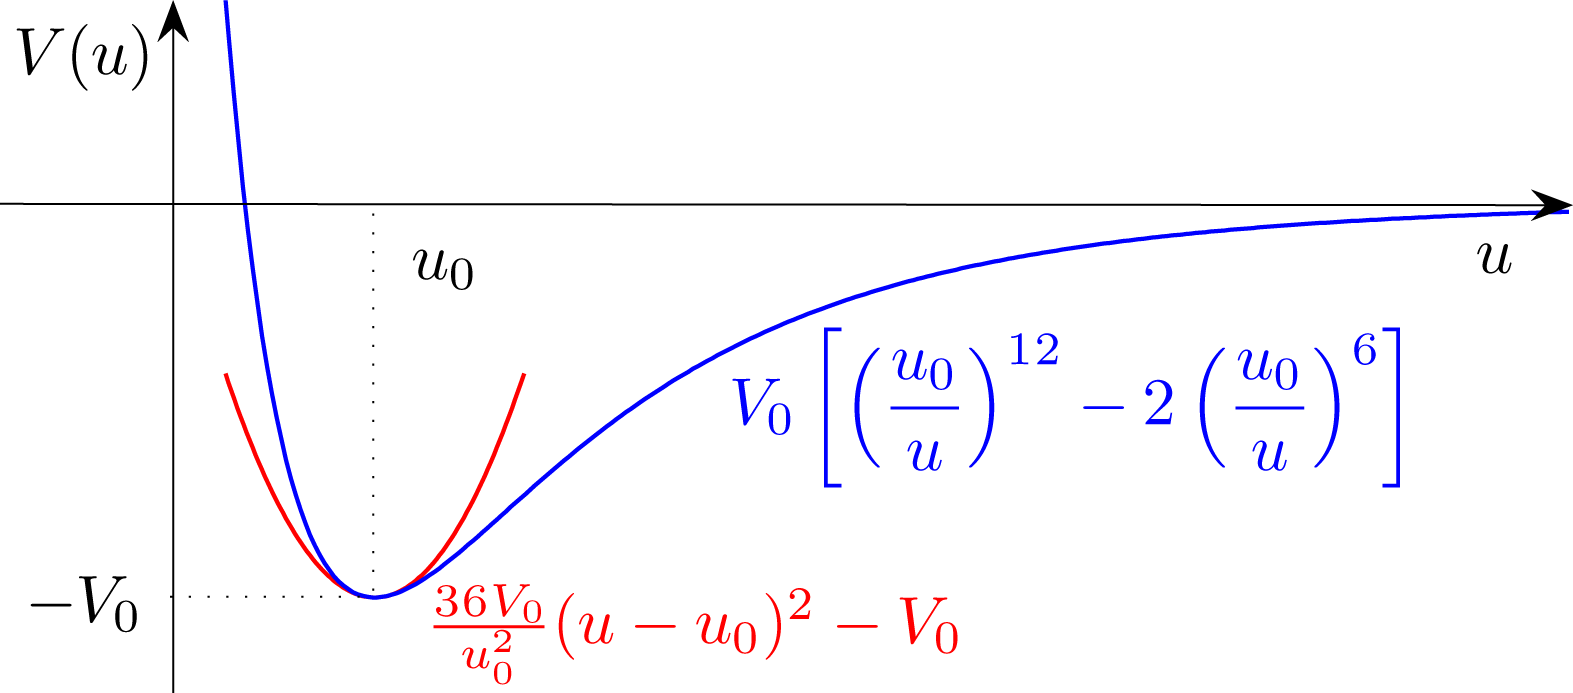
\includegraphics[width=6cm]{image/5-3-6.png}
\caption{范氏等温线}
\end{wrapfigure}
考虑了分子间作用力的\emph{范德瓦尔斯方程}(van der Waals equation), 其形式为:
\[\left(p+\frac{\nu^2 a}{V^2}\right)(V-\nu b)=\nu RT\]

其等温线形状如图所示. 或者取一摩尔气体, 压强作为摩尔体积$v$的函数为
\[p=\frac{RT}{v-b}-\frac{a}{v^2}\]

这么一个简单的方程中蕴藏着气液相变的精髓, 实际上直到今天我们对气液相变的理解也不比范德瓦尔斯方程所预示的高明多少.

首先注意到, 高温时范德瓦尔斯等温线接近理想气体的等温线. 但是当温度在$T_c$以下时, 其等温线开始出现斜率等于零的点和正斜率的曲线段. 而\emph{临界温度}(critical temperature)$T_c$对应的等温线只有一个斜率等于零的点$K$, 称为\emph{临界点}(critical point). 这个点曲线的一阶和二阶导数应当同时为零, 简单的计算可以给出:
\[T_c= \frac{8a}{27Rb} \quad,\quad p_c=\frac{a}{27 b^2} \quad,\quad v_c=3b\]

\begin{wrapfigure}[17]{o}[-10pt]{6cm}
\centering
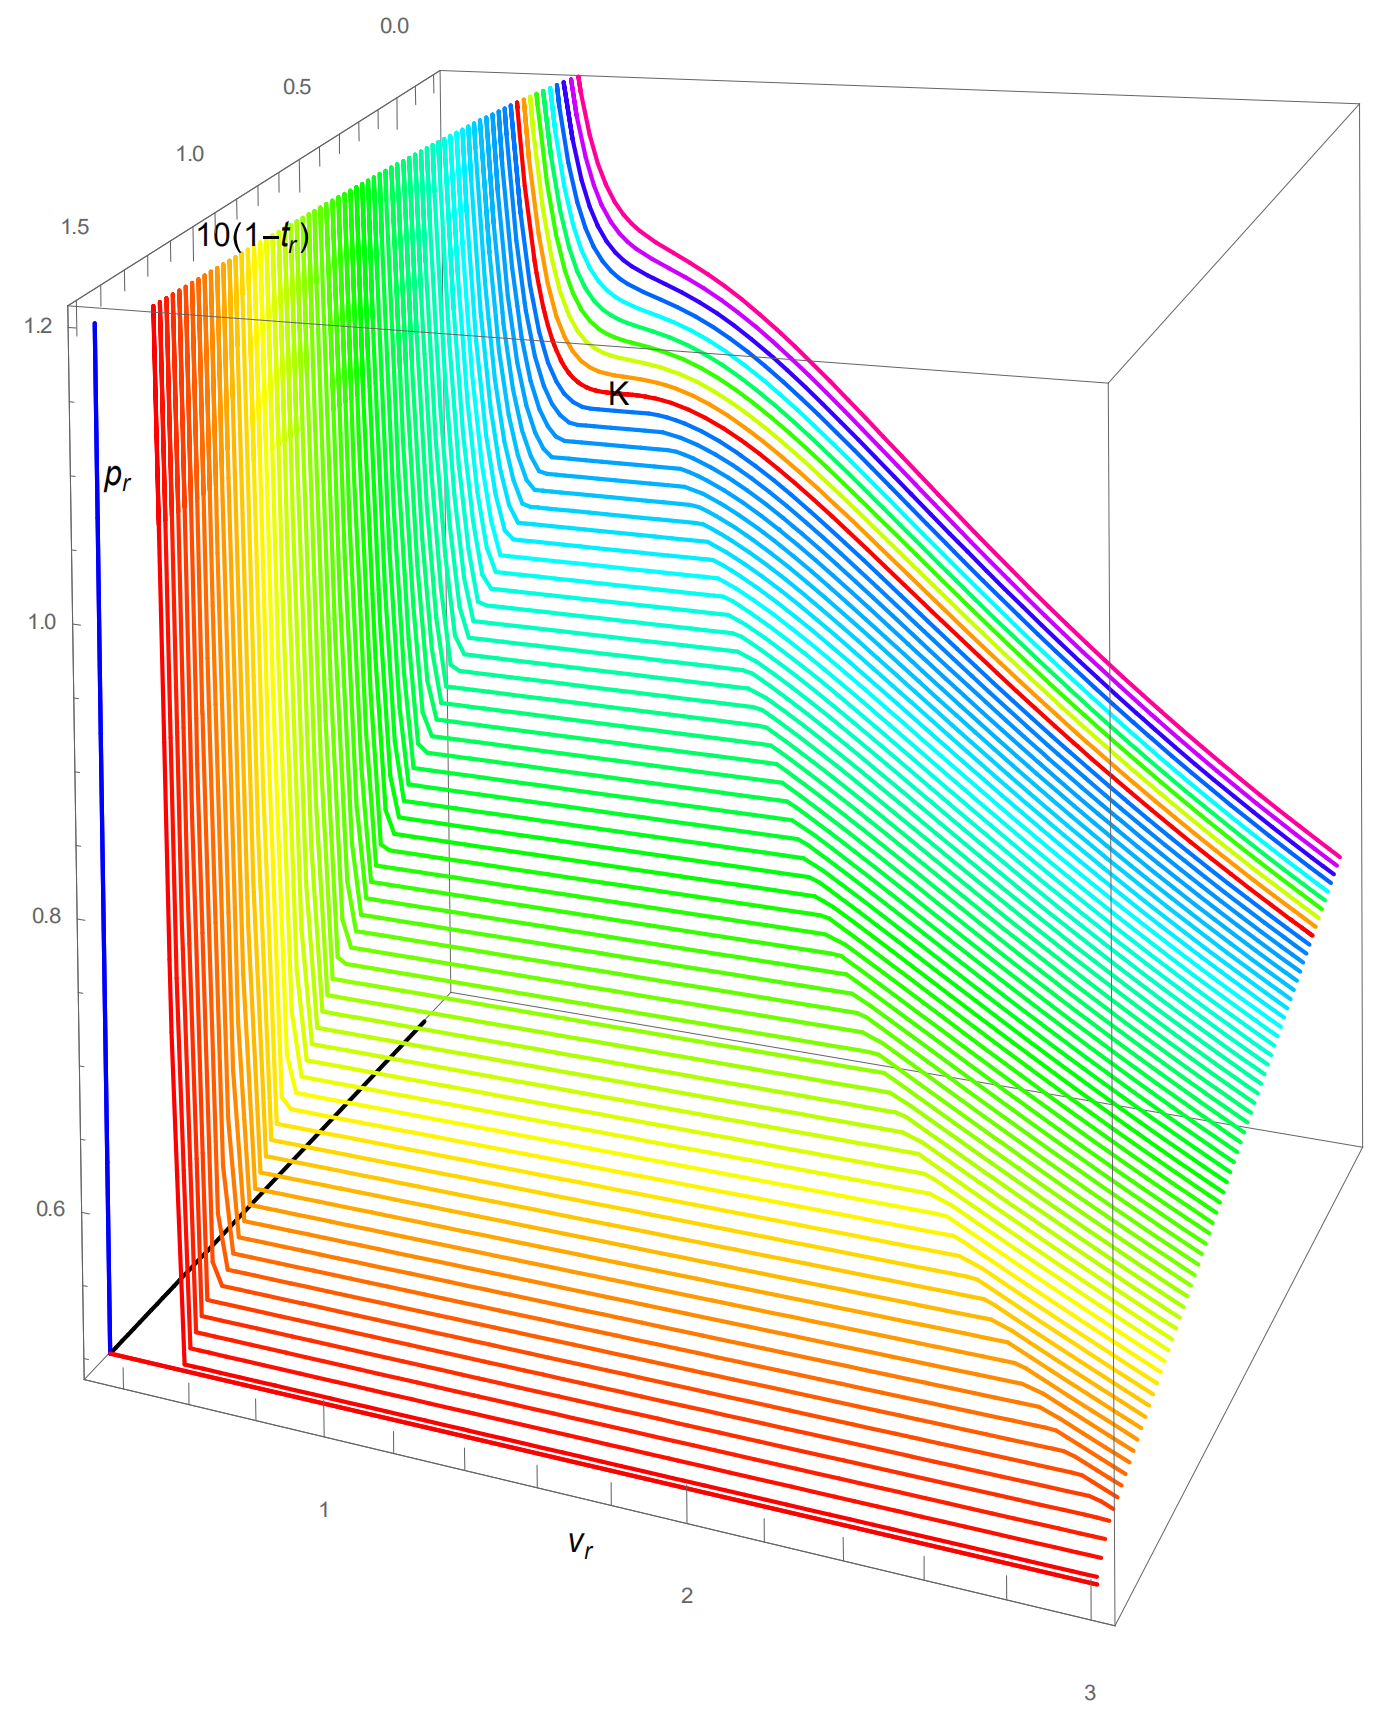
\includegraphics[width=6cm]{image/5-3-9.png}
\caption{气液相变状态空间}
\end{wrapfigure}历史上麦克斯韦第一次指出, 低于临界温度时, 曲线上存在两个点$b,\,c$如上图, $b$点对应两相平衡时的液态, 而$c$对应两相平衡时的气态. 两相恰好可以平衡共存. 而两者之间两阴影部分面积需要相等, 称作\emph{等面积法则}(rule of equal areas). 我们今天可以如下来理解这个结论. 考虑平衡共存时的三个条件, 现在$b,\,c$在同一条等温线上且压强相等, 热学平衡和力学平衡已经达成. 接下来只需要化学平衡, 即:
\[\mu_b=\mu_c\]

而根据化学势的微分公式:
\[\ud \mu=-s\ud T +v\ud p\]

故若沿等温线从$b$状态到$c$状态:
\[\mu_b-\mu_c=0=\int_b^c v\ud p\]

这个等式足以说明麦克斯韦等面积法则. 为了更加直观, 我们使用分布积分, 并记$b,\,c$压强为$p$:
\[p(v_c-v_b)-\int_b^c p\ud v=0\]


这就是说$bc$间直线下方面积等于$bc$间曲线下方的面积, 从而两阴影部分面积相等.




%\section{连续相变}

%\section{拓扑相变}